\documentclass{standalone}
\usepackage{xcolor}
\usepackage{tikz}
\usetikzlibrary{positioning, shapes.multipart, calc, graphs, graphs.standard}
\begin{document}
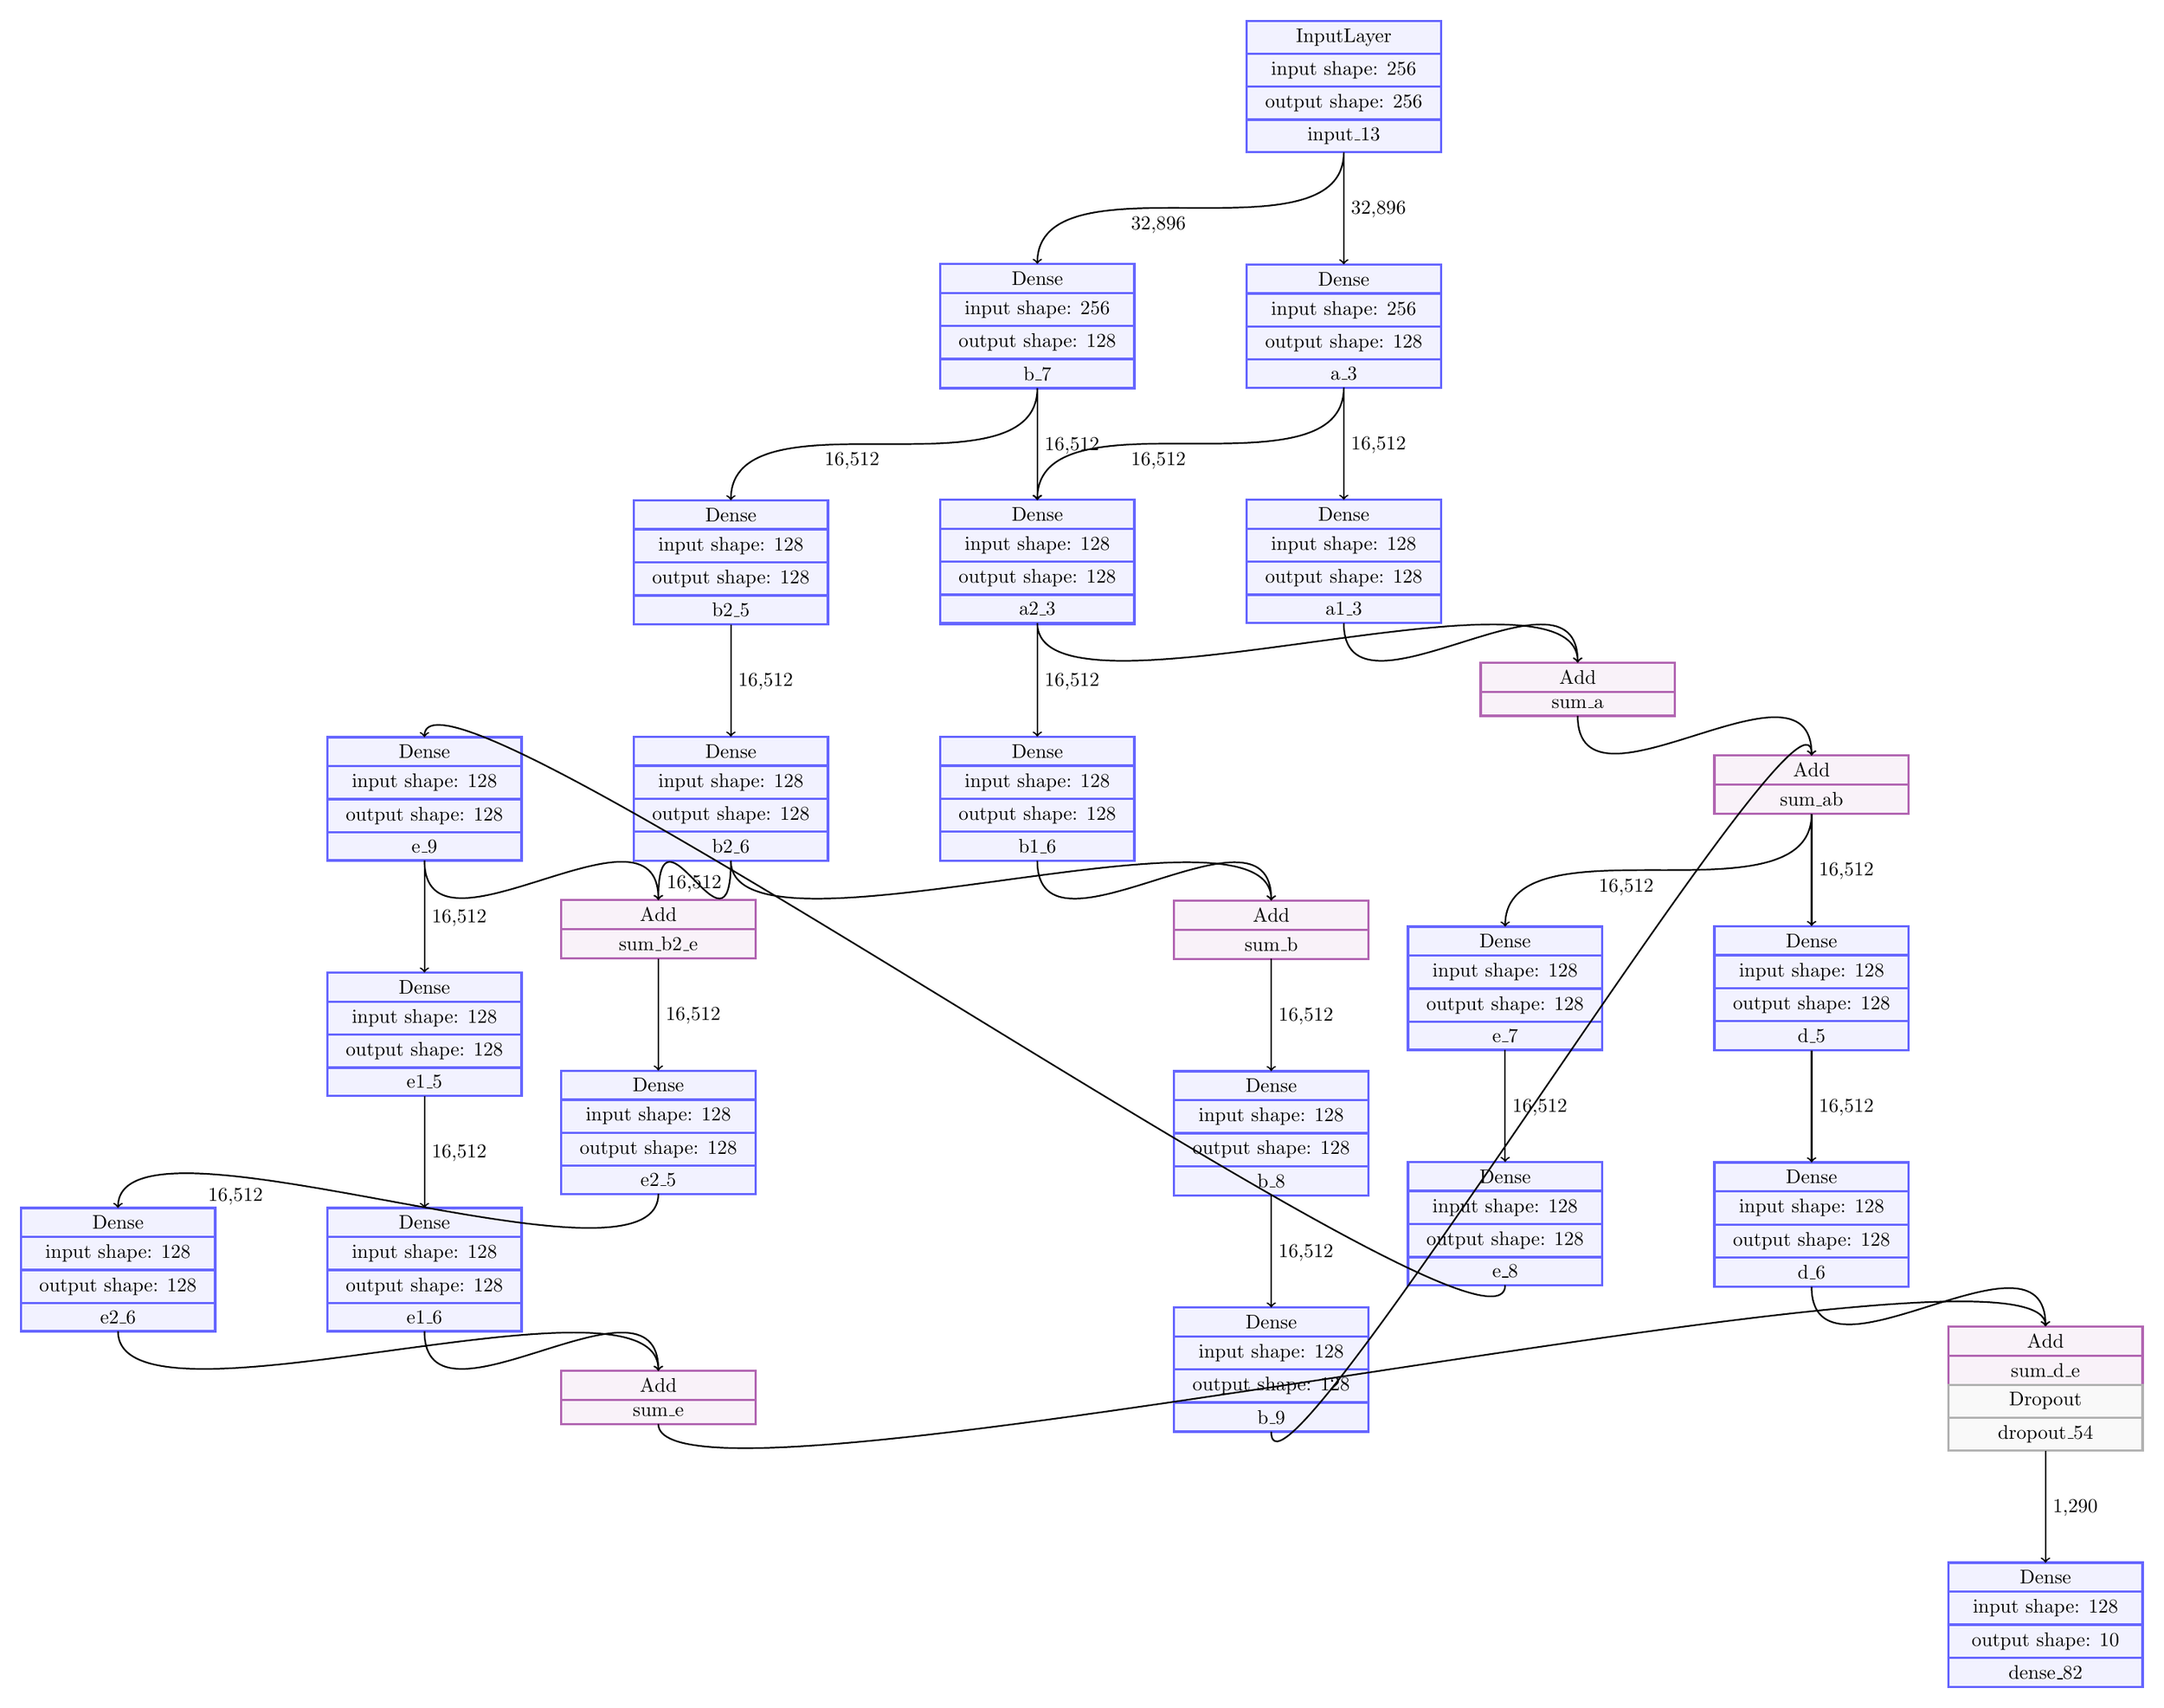
\begin{tikzpicture}
[default_edge/.style={thick,out=-90,in=90,out distance=2cm,in distance=2cm},default_label/.style={auto,pos=0.65},TrainableLayer_style/.style={rectangle split,rectangle split ignore empty parts,very thick,rectangle split parts=10,draw=blue!60,fill=blue!5,minimum width={width("Batch Normalisation") + 8pt},node distance=2cm,outer sep=0cm},OperationLayer_style/.style={rectangle split,rectangle split ignore empty parts,very thick,rectangle split parts=10,draw=violet!60,fill=violet!5,minimum width={width("Batch Normalisation") + 8pt},node distance=1cm,outer sep=0cm},UtilityLayer_style/.style={rectangle split,rectangle split ignore empty parts,very thick,rectangle split parts=10,draw=gray!60,fill=gray!5,minimum width={width("Batch Normalisation") + 8pt},node distance=0cm,outer sep=0cm}]
\node[TrainableLayer_style] [] (input_13) {\nodepart{one}{InputLayer}\nodepart{two}{input shape: 256}\nodepart{three}{output shape: 256}\nodepart{four}{input\_13}};
\node[TrainableLayer_style] [below=of input_13] (a_3) {\nodepart{one}{Dense}\nodepart{two}{input shape: 256}\nodepart{three}{output shape: 128}\nodepart{four}{a\_3}};
\node[TrainableLayer_style] [below=of input_13,left=of a_3] (b_7) {\nodepart{one}{Dense}\nodepart{two}{input shape: 256}\nodepart{three}{output shape: 128}\nodepart{four}{b\_7}};
\node[TrainableLayer_style] [below=of b_7] (b1_5) {\nodepart{one}{Dense}\nodepart{two}{input shape: 128}\nodepart{three}{output shape: 128}\nodepart{four}{b1\_5}};
\node[TrainableLayer_style] [below=of b1_5] (b1_6) {\nodepart{one}{Dense}\nodepart{two}{input shape: 128}\nodepart{three}{output shape: 128}\nodepart{four}{b1\_6}};
\node[TrainableLayer_style] [below=of a_3] (a1_3) {\nodepart{one}{Dense}\nodepart{two}{input shape: 128}\nodepart{three}{output shape: 128}\nodepart{four}{a1\_3}};
\node[TrainableLayer_style] [below=of b_7,left=of b1_5] (b2_5) {\nodepart{one}{Dense}\nodepart{two}{input shape: 128}\nodepart{three}{output shape: 128}\nodepart{four}{b2\_5}};
\node[TrainableLayer_style] [below=of a_3,left=of a1_3] (a2_3) {\nodepart{one}{Dense}\nodepart{two}{input shape: 128}\nodepart{three}{output shape: 128}\nodepart{four}{a2\_3}};
\node[TrainableLayer_style] [below=of b2_5,left=of b1_6] (b2_6) {\nodepart{one}{Dense}\nodepart{two}{input shape: 128}\nodepart{three}{output shape: 128}\nodepart{four}{b2\_6}};
\node[OperationLayer_style] [below right=of b1_6] (sum_b) {\nodepart{one}{Add}\nodepart{two}{sum\_b}};
\node[OperationLayer_style] [below right=of a1_3] (sum_a) {\nodepart{one}{Add}\nodepart{two}{sum\_a}};
\node[TrainableLayer_style] [below=of sum_b] (b_8) {\nodepart{one}{Dense}\nodepart{two}{input shape: 128}\nodepart{three}{output shape: 128}\nodepart{four}{b\_8}};
\node[TrainableLayer_style] [below=of b_8] (b_9) {\nodepart{one}{Dense}\nodepart{two}{input shape: 128}\nodepart{three}{output shape: 128}\nodepart{four}{b\_9}};
\node[OperationLayer_style] [below right=of sum_a] (sum_ab) {\nodepart{one}{Add}\nodepart{two}{sum\_ab}};
\node[TrainableLayer_style] [below=of sum_ab] (d_5) {\nodepart{one}{Dense}\nodepart{two}{input shape: 128}\nodepart{three}{output shape: 128}\nodepart{four}{d\_5}};
\node[TrainableLayer_style] [below=of sum_ab,left=of d_5] (e_7) {\nodepart{one}{Dense}\nodepart{two}{input shape: 128}\nodepart{three}{output shape: 128}\nodepart{four}{e\_7}};
\node[TrainableLayer_style] [below=of e_7] (e_8) {\nodepart{one}{Dense}\nodepart{two}{input shape: 128}\nodepart{three}{output shape: 128}\nodepart{four}{e\_8}};
\node[TrainableLayer_style] [below=of e_8,left=of b2_6] (e_9) {\nodepart{one}{Dense}\nodepart{two}{input shape: 128}\nodepart{three}{output shape: 128}\nodepart{four}{e\_9}};
\node[TrainableLayer_style] [below=of e_9] (e1_5) {\nodepart{one}{Dense}\nodepart{two}{input shape: 128}\nodepart{three}{output shape: 128}\nodepart{four}{e1\_5}};
\node[TrainableLayer_style] [below=of e1_5] (e1_6) {\nodepart{one}{Dense}\nodepart{two}{input shape: 128}\nodepart{three}{output shape: 128}\nodepart{four}{e1\_6}};
\node[TrainableLayer_style] [below=of d_5] (d_6) {\nodepart{one}{Dense}\nodepart{two}{input shape: 128}\nodepart{three}{output shape: 128}\nodepart{four}{d\_6}};
\node[OperationLayer_style] [below right=of e_9] (sum_b2_e) {\nodepart{one}{Add}\nodepart{two}{sum\_b2\_e}};
\node[TrainableLayer_style] [below=of sum_b2_e] (e2_5) {\nodepart{one}{Dense}\nodepart{two}{input shape: 128}\nodepart{three}{output shape: 128}\nodepart{four}{e2\_5}};
\node[TrainableLayer_style] [below=of e2_5,left=of e1_6] (e2_6) {\nodepart{one}{Dense}\nodepart{two}{input shape: 128}\nodepart{three}{output shape: 128}\nodepart{four}{e2\_6}};
\node[OperationLayer_style] [below right=of e1_6] (sum_e) {\nodepart{one}{Add}\nodepart{two}{sum\_e}};
\node[OperationLayer_style] [below right=of d_6] (sum_d_e) {\nodepart{one}{Add}\nodepart{two}{sum\_d\_e}};
\draw[->, default_edge] (input_13) to node [default_label] {32,896} (b_7);
\node[UtilityLayer_style] [below=of sum_d_e] (dropout_54) {\nodepart{one}{Dropout}\nodepart{two}{dropout\_54}};
\draw[->, default_edge] (b_7) to node [default_label] {16,512} (b1_5);
\node[TrainableLayer_style] [below=of dropout_54] (dense_82) {\nodepart{one}{Dense}\nodepart{two}{input shape: 128}\nodepart{three}{output shape: 10}\nodepart{four}{dense\_82}};
\draw[->, default_edge] (b_7) to node [default_label] {16,512} (b2_5);
\draw[->, default_edge] (b1_5) to node [default_label] {16,512} (b1_6);
\draw[->, default_edge] (b2_5) to node [default_label] {16,512} (b2_6);
\draw[->, default_edge] (input_13) to node [default_label] {32,896} (a_3);
\draw[->, default_edge] (b1_6) to node [default_label] {} (sum_b);
\draw[->, default_edge] (b2_6) to node [default_label] {} (sum_b);
\draw[->, default_edge] (a_3) to node [default_label] {16,512} (a1_3);
\draw[->, default_edge] (a_3) to node [default_label] {16,512} (a2_3);
\draw[->, default_edge] (sum_b) to node [default_label] {16,512} (b_8);
\draw[->, default_edge] (a1_3) to node [default_label] {} (sum_a);
\draw[->, default_edge] (a2_3) to node [default_label] {} (sum_a);
\draw[->, default_edge] (b_8) to node [default_label] {16,512} (b_9);
\draw[->, default_edge] (sum_a) to node [default_label] {} (sum_ab);
\draw[->, default_edge] (b_9) to node [default_label] {} (sum_ab);
\draw[->, default_edge] (sum_ab) to node [default_label] {16,512} (e_7);
\draw[->, default_edge] (e_7) to node [default_label] {16,512} (e_8);
\draw[->, default_edge] (e_8) to node [default_label] {16,512} (e_9);
\draw[->, default_edge] (e_9) to node [default_label] {} (sum_b2_e);
\draw[->, default_edge] (b2_6) to node [default_label] {} (sum_b2_e);
\draw[->, default_edge] (e_9) to node [default_label] {16,512} (e1_5);
\draw[->, default_edge] (sum_b2_e) to node [default_label] {16,512} (e2_5);
\draw[->, default_edge] (sum_ab) to node [default_label] {16,512} (d_5);
\draw[->, default_edge] (e1_5) to node [default_label] {16,512} (e1_6);
\draw[->, default_edge] (e2_5) to node [default_label] {16,512} (e2_6);
\draw[->, default_edge] (d_5) to node [default_label] {16,512} (d_6);
\draw[->, default_edge] (e1_6) to node [default_label] {} (sum_e);
\draw[->, default_edge] (e2_6) to node [default_label] {} (sum_e);
\draw[->, default_edge] (d_6) to node [default_label] {} (sum_d_e);
\draw[->, default_edge] (sum_e) to node [default_label] {} (sum_d_e);
\draw[->, default_edge] (dropout_54) to node [default_label] {1,290} (dense_82);
\end{tikzpicture}\end{document}